% !TeX root = main.tex
% !LW recipe = latexmk (presentation)
\documentclass[aspectratio=169,11pt,t]{beamer}
\usepackage{beamart}
\usepackage{quantikz}

\title{Simulating magic in quantum error correction}
\presenter{Arthur Pesah}{FU Berlin}
\date{}
\venue{}
\coauthors{%
  \coauthorportrait[yshift=-3mm]{assets/serban-cercelescu.png}
    {Serban Cercelescu}{Oxford}%
  \hspace{9mm}%
  \coauthorportrait[yshift=-4.5mm]{assets/mark-koch.jpg}{Mark Koch}{Oxford}%
}
\hypersetup{pdfauthor={Arthur Pesah},
  pdftitle={When can magic be easy to simulate?},
  pdfsubject={Efficiently benchmarking quantum error correction}}

\arxivpaper[assets/qr-arxiv-transparent.png]{2610.06811}
\githubrepo[assets/qr-github-transparent.png]{mark-koch}{merlin-sim}

% Keep the resource layout from beamart, adding the subtitle only for this talk.
\setbeamertemplate{title page}{%
  \begin{tikzpicture}[remember picture,overlay]
    \begin{scope}[shift={(current page.north west)},x=1mm,y=1mm]
      \node[align=center,text width=.92\paperwidth,inner sep=0pt]
        at (80,-14)
        {{\usebeamerfont{title}\color{DCPAccent}\inserttitle\par}};
      \node[align=center,text width=.92\paperwidth,inner sep=0pt,
        text=DCPMuted,font=\fontsize{11}{14}\selectfont]
        at (80,-25) {\insertsubtitle};
      \node[align=center,text width=76mm,inner sep=0pt] at (80,-37)
        {{\fontsize{15}{19}\selectfont\bfseries\DCPPresenterName\par}
         \vspace{1mm}
         {\fontsize{11}{14}\selectfont\color{DCPMuted}\DCPPresenterAffiliation\par}};
      \node[text=DCPMuted,font=\fontsize{9}{11}\selectfont]
        at (80,-49) {Joint work with};
      \node[inner sep=0pt] at (80,-68)
        {\begingroup\tikzset{x=1cm,y=1cm}\scalebox{.8}{\DCPCoauthors}\endgroup};
      \resourcecard{22}{\faGithub\ GitHub}{\DCPGithubOwner/\\\DCPGithubRepo}
        {\DCPGithubURL}{\DCPGithubQR}
      \resourcecard{138}{\aiarXiv\ arXiv}{\DCPArxivID}
        {\DCPArxivURL}{\DCPArxivQR}
    \end{scope}
  \end{tikzpicture}%
}

\definecolor{CodeBlue}{HTML}{356C9B}
\definecolor{CodeGreen}{HTML}{00836B}
\definecolor{CodePurple}{HTML}{86519B}
\definecolor{BitError}{HTML}{B53D36}
\newcommand{\wordone}[1]{{\color{CodeBlue}#1}}
\newcommand{\wordtwo}[1]{{\color{CodeGreen}#1}}
\newcommand{\wordthree}[1]{{\color{CodePurple}#1}}
\newcommand{\flippedbit}[1]{{\color{BitError}\underline{\mathbf{#1}}}}
\newcommand{\messagebits}{\wordone{0}\wordtwo{1}\wordthree{1}}
\newcommand{\encodedbits}{\wordone{000}\,\wordtwo{111}\,\wordthree{111}}
\newcommand{\noisybits}{\wordone{0\flippedbit{1}0}\,\wordtwo{1\flippedbit{0}1}\,\wordthree{111}}

\begin{document}

% Target speaking time: 0:20.
\begin{frame}
  \titlepage
  \note{The question in the title has a practical motivation. We want to compare
    ways to protect quantum computations, including the ingredients usually
    associated with hard classical simulation.}
\end{frame}

% Target speaking time: 1:10.
\begin{frame}{What quantum circuits are classically simulable?}
  \centering
  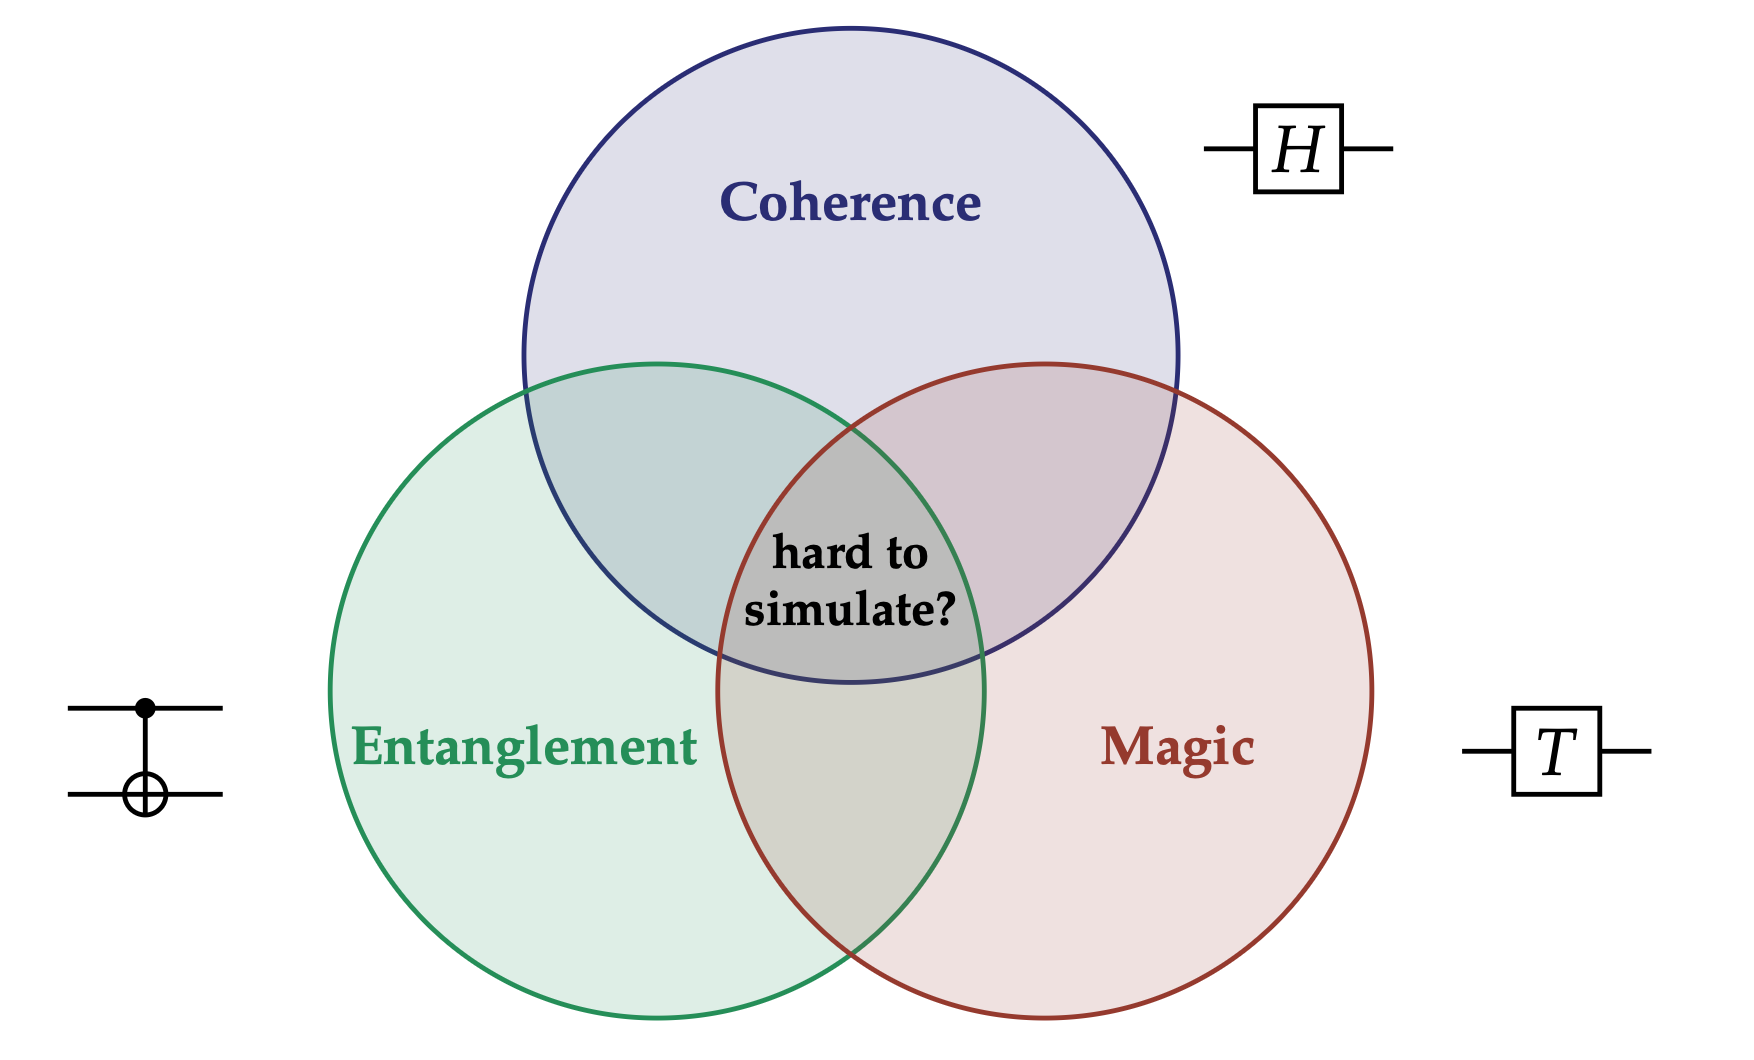
\includegraphics[height=.51\paperheight]{assets/venn-diagram.png}\par
  \vspace{-2mm}
  \uncover<2->{\emphword{Magic}: non-Clifford ingredients, such as $T$ gates.\par}
  \uncover<3->{The answer has practical consequences for \emphword{quantum error correction}.\par}
  \note{The diagram is a way to ask the question, not a complete classification.
    Entanglement alone is not enough to make a circuit hard to simulate. Even
    the presence of all three ingredients does not automatically imply hardness.
    Explain magic as a name for ingredients that take us beyond Clifford
    circuits, with the T gate as the example.}
\end{frame}

% Target speaking time: 1:20, including the classical example.
\begin{frame}{Quantum error correction}
  \emphword{The idea}: add redundancy to protect information against errors.

  \uncover<2->{%
    \emphword{Classical example}: repeat each bit three times.
    \[
      \renewcommand{\arraystretch}{1.05}
      \begin{array}{r@{\quad}c@{\quad}l}
        \messagebits & \xrightarrow{\text{encode}} & \encodedbits \\
        \multicolumn{2}{c}{} &
          \uncover<3->{\hspace{7mm}\Big\downarrow\;{\scriptstyle\text{two bit flips}}} \\
        \uncover<4->{\messagebits} &
          \uncover<4->{\xleftarrow{\text{majority vote}}} &
          \uncover<3->{\noisybits}
      \end{array}
    \]
  }
  \uncover<5->{\par\noindent
    \emphword{Quantum version}: encode each logical qubit across several physical qubits.\\
    Measure error checks without reading out the stored information.
    \par
  }
  \note{Read 011 as a classical message of three bits. Its encoding is
    000111111, with colours separating the three codewords. The two red,
    underlined bits have flipped. Each affected block still has the correct
    majority, so decoding recovers 011. This code corrects one bit flip per
    block, not two arbitrary errors in one block. Quantum information cannot
    simply be copied. The quantum version distributes it across an encoded
    state and extracts information about errors.}
\end{frame}

% Target speaking time: 1:30.
\begin{frame}{Gates on encoded qubits}
  \setlength{\parskip}{3bp}
  Each gate in the algorithm needs a \emphword{fault-tolerant logical implementation}.

  \begin{columns}[T,onlytextwidth]
    \begin{column}{.19\textwidth}
      \centering
      \strut\emphword{Algorithm}\par
      \vspace{2mm}
      \begin{minipage}[c][38mm][c]{\linewidth}
        \centering
        \begin{quantikz}[column sep=3mm]
          & \gate[style={fill=none}]{H} & \qw
        \end{quantikz}
      \end{minipage}
    \end{column}
    \begin{column}{.06\textwidth}
      \centering
      \strut\par
      \vspace{2mm}
      \begin{minipage}[c][38mm][c]{\linewidth}
        \centering
        \uncover<2->{\Large$\longrightarrow$}
      \end{minipage}
    \end{column}
    \begin{column}{.75\textwidth}
      \centering
      \uncover<2->{%
        \strut\emphword{Encoded implementation}\par
        \vspace{2mm}
        % Wire 2 carries the unlabelled logical input. The labelled ancilla on
        % wire 1 starts in plus, and those on wires 3 and 4 start in zero.
        % This encoder
        % fixes the unused logical qubit to zero. The final H layer and SWAP
        % apply H to the displayed qubit and change the unused logical state.
        % For arbitrary values on both logical inputs, add CNOT 3 -> 4 before
        % the three CNOTs controlled by wire 1 to obtain the full CSS encoder.
        \begin{minipage}[c][38mm][c]{\linewidth}
        \centering
        \begin{quantikz}[column sep=2.7mm,row sep=3.1mm,
          cells={nodes={font=\small}}]
          \lstick{$\ket{+}$} & \qw\gategroup[wires=4,steps=4,
              style={dashed,draw=DCPAccent!55,rounded corners=1pt,
                inner xsep=3pt,inner ysep=4pt},
              label style={label position=below,anchor=north,yshift=-1mm}]
              {\scriptsize Encoding}
            & \ctrl{1} & \ctrl{2} & \ctrl{3}
            & \gate[style={fill=none}]{H} & \qw      & \qw \\
          & \ctrl{2} & \targ{}  & \qw      & \qw
            & \gate[style={fill=none}]{H} & \swap{1} & \qw \\
          \lstick{$\ket{0}$} & \qw & \qw & \targ{} & \qw
            & \gate[style={fill=none}]{H} & \targX{} & \qw \\
          \lstick{$\ket{0}$} & \targ{} & \qw & \qw & \targ{}
            & \gate[style={fill=none}]{H} & \qw      & \qw
        \end{quantikz}
        \end{minipage}\par
      }
    \end{column}
  \end{columns}
  \vspace{1mm}
  \uncover<3->{A small circuit becomes a \emphword{larger circuit on more qubits}.}
  \note{The circuit illustrates encoding overhead and a logical gate.
    Single-qubit gates applied in parallel do not spread a fault between
    qubits. The four-qubit code detects a single-qubit error, rather than
    correcting it without further resources. The simple encoder is an
    illustration of encoding, not a complete fault-tolerant preparation and
    error-correction protocol. Full protocols add checks and often ancillas.}
\end{frame}

% Target speaking time: 1:20.
\begin{frame}{Benchmarking quantum error correction}
  A protocol converts physical errors into a logical error rate:
  \vspace{2mm}
  \[
    \underbrace{\epsilon}_{\substack{\text{error probability}\\\text{per physical operation}}}
    \quad\xrightarrow{\quad\text{QEC protocol}\quad}\quad
    \underbrace{\epsilon_L}_{\substack{\text{failure probability}\\\text{of the logical operation}}}
  \]
  \vspace{2mm}
  \pause
  \emphword{Goal}: make $\epsilon_L$ as small as possible at an affordable cost.

  \pause
  \emphword{How?} Simulate noisy protocols, count logical failures, and compare designs.
  \note{The mapping depends on the protocol, noise model, and resources.
    Compare candidate protocols under a common noise model and account for
    their cost. For protocols that reject runs when errors are detected,
    acceptance probability is another important quantity. A lower conditional
    error rate alone is not enough to decide which protocol is better.}
\end{frame}

% Target speaking time: 1:10.
\begin{frame}{The simulation bottleneck}
  \begin{itemize}
    \item \emphword{Clifford circuits}: efficient classical simulation, even with many qubits.
    \pause
    \item Universal quantum computing also needs \emphword{non-Clifford ingredients},
      often supplied as magic states.
    \pause
    \item Generic simulation methods can become \emphword{exponentially costly}
      as magic increases.
  \end{itemize}

  \pause
  \emphword{Until our work}: only \emphword{small-scale} benchmarking of logical magic protocols possible.

  \pause
  Can we exploit the structure of quantum error correction?
  \note{This is a limitation of generic methods, not a claim that no logical
    magic protocol could previously be simulated. Previous approaches had
    different costs and restrictions. The question is whether the structure
    needed for error correction makes useful families easier to simulate.}
\end{frame}

% Target speaking time: 2:00. Planned content: 8:50, leaving time for transitions.
\begin{frame}{Efficient simulation of quantum error correction}
  \begin{itemize}
    \item QEC implementations of magic gates have \emphword{structure we can exploit}.
    \pause
    \item For a broad class of these protocols, we obtain \emphword{polynomial-time classical simulation}.
    \pause
    \item \emphword{MERLIN}: our open-source simulator for benchmarking logical magic protocols.
  \end{itemize}

  \pause
  \emphword{If magic alone is not enough, what makes quantum circuits hard to simulate?}
  \paperlinks
  \pause
  \vspace{6mm}
  \begin{center}
    {\usebeamerfont{title}\emphword{Thanks!}}
  \end{center}
  \note{The key observation is that QEC implementations of magic gates are
    structured circuits. We exploit that structure to simulate a broad class
    of useful protocols efficiently, including noise within the model covered
    by our result. MERLIN makes this method available for practical benchmarking.
    Efficient simulation of each run still leaves the sampling cost of
    estimating rare logical errors. Close with the foundational question:
    magic can be present in an efficiently simulable circuit, so what features
    of a quantum computation determine its classical simulation cost? Point
    to the paper and code links for the details.}
\end{frame}

\end{document}
